\documentclass[tikz,border=6pt]{standalone}
\usepackage{amsmath,amssymb,mathtools,physics,bm,nicefrac,wasysym}
\usepackage{xcolor}

\definecolor{colone}{RGB}{180,60,60}
\definecolor{coltwo}{RGB}{60,110,180}
\definecolor{colthree}{RGB}{60,140,80}

\definecolor{accent}{HTML}{A13D2C}
\definecolor{accent2}{HTML}{2B5F6B}
\definecolor{muted}{HTML}{5A564F}
\definecolor{panel}{HTML}{F8F6F0}
\definecolor{linecol}{HTML}{D8D2C4}
\definecolor{ink}{HTML}{1E1C1A}
\definecolor{astroblue}{HTML}{1B4F72}
\definecolor{astrodark}{HTML}{17202A}
\definecolor{sunyellow}{HTML}{E8A33D}

\usetikzlibrary{calc,arrows.meta,positioning,decorations.pathreplacing,decorations.markings,angles,quotes,shapes.geometric}
\usepackage{tikz-3dplot}

\newcommand{\vecr}{\vec r}
\newcommand{\vecL}{\vec L}
\newcommand{\vecA}{\vec A}
\newcommand{\vecf}{\vec f}
\newcommand{\vecF}{\vec F}
\newcommand{\vecp}{\vec p}
\newcommand{\avg}[1]{\left\langle #1\right\rangle}
\newcommand{\vecx}{\vec x}
\newcommand{\hatn}{\hat n}
\newcommand{\rhat}{\hat r}
\newcommand{\phihat}{\hat\phi}
\newcommand{\thetahat}{\hat\theta}
\newcommand{\note}[1]{\textcolor{blue!60!black}{\textit{[#1]}}}

% Astronomical acronyms
\newcommand{\LST}{\mathrm{LST}}
\newcommand{\GST}{\mathrm{GST}}
\newcommand{\GMST}{\mathrm{GMST}}
\newcommand{\GAST}{\mathrm{GAST}}
\newcommand{\LMST}{\mathrm{LMST}}
\newcommand{\LAST}{\mathrm{LAST}}
\newcommand{\UT}{\mathrm{UT}}
\newcommand{\UTC}{\mathrm{UTC}}
\newcommand{\TAI}{\mathrm{TAI}}
\newcommand{\TT}{\mathrm{TT}}
\newcommand{\TDB}{\mathrm{TDB}}
\newcommand{\JD}{\mathrm{JD}}
\newcommand{\MJD}{\mathrm{MJD}}
\newcommand{\EoT}{\mathrm{EoT}}
\newcommand{\SNR}{\mathrm{SNR}}
\newcommand{\RON}{\mathrm{RON}}

% Helper commands for specific diagrams
\newcommand{\midlinelabel}[3]{
    \node (midlabel) at ($ (#1)!.5!(#2) $) {#3};
    \draw[stealth-] (#1) --  (midlabel);
    \draw[-stealth] (midlabel) -- (#2);
}
\newcommand{\midlinelabell}[3]{
    \node[fill = white, inner sep = 0.2pt, outer sep=3pt] (midlabel) at ($ (#1)!.5!(#2) $) {#3};
    \draw[stealth-] (#1) --  (midlabel);
    \draw[-stealth] (midlabel) -- (#2);
}
\newcommand{\midlinelabelll}[3]{
    \node[fill = white, inner sep = 0.2pt, outer sep=3pt,scale=0.6] (midlabel) at ($ (#1)!.5!(#2) $) {#3};
    \draw[stealth-] (#1) --  (midlabel);
    \draw[-stealth] (midlabel) -- (#2);
}



\begin{document}
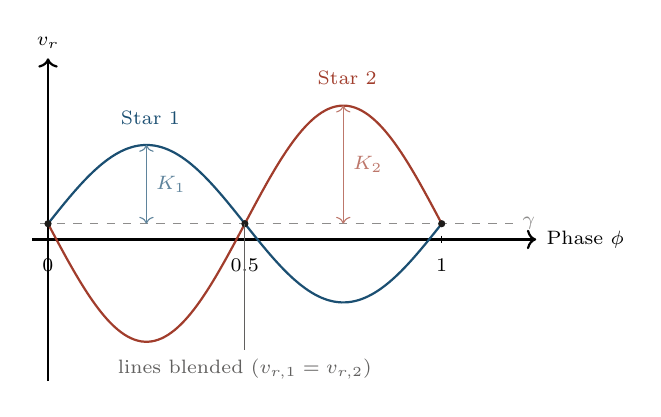
\begin{tikzpicture}[font=\scriptsize]
			% Axes
			\draw[->, thick] (-0.2,0) -- (6.2,0) node[right] {Phase $\phi$};
			\draw[->, thick] (0,-1.8) -- (0,2.3) node[above] {$v_r$};
			\foreach \p/\lab in {0/0, 2.5/0.5, 5/1} {
				\draw (\p,0.05) -- (\p,-0.05) node[below=2pt] {\lab};
			}

			% Systemic velocity
			\draw[ink!50, dashed] (-0.1,0.2) -- (5.9,0.2) node[right] {$\gamma$};

			% v1 = gamma + K1 sin(2 pi phase), K1 = 1.0
			\draw[astroblue, thick, domain=0:1, samples=60, smooth, variable=\p]
				plot ({5*\p}, {0.2 + 1.0*sin(360*\p)});
			% v2 = gamma - K2 sin(2 pi phase), K2 = 1.5
			\draw[accent, thick, domain=0:1, samples=60, smooth, variable=\p]
				plot ({5*\p}, {0.2 - 1.5*sin(360*\p)});

			% Amplitude brackets, both read off at quadrature phases
			\draw[<->, astroblue!70] (1.25,0.2) -- (1.25,1.2) node[midway, right] {$K_1$};
			\draw[<->, accent!70] (3.75,0.2) -- (3.75,1.7) node[midway, right] {$K_2$};

			% Lines-blended crossings, where v_{r,1}=v_{r,2}
			\foreach \xc in {0,2.5,5}{
				\fill[ink] (\xc,0.2) circle (1.3pt);
			}
			\draw[ink!70, thin] (2.5,0.2) -- (2.5,-1.4);
			\node[ink!70, align=center] at (2.5,-1.65) {lines blended ($v_{r,1}=v_{r,2}$)};

			\node[astroblue] at (1.3,1.55) {Star 1};
			\node[accent] at (3.8,2.05) {Star 2};
		\end{tikzpicture}
\end{document}
